\documentclass{article}
\usepackage[T1]{fontenc}
\usepackage[section]{placeins}
\usepackage{graphicx}
\usepackage[font=small,labelfont=bf]{caption}
\usepackage[scale=1]{tgheros} % or helvet
\renewcommand{\familydefault}{\sfdefault}

\begin{document}
\title{Proposal for SynerGE HealthCare, 2019}


\author{ 
	Damodar Nayak  \\ \and 
	Rohit Sarkar  \\  \and
	Yash Raj Sarrof }
\date{}

% Let's get started

\maketitle



% Section and subsections will appear in the presentation overview
% and table of contents.
\section*{Detailed Idea}

\subsection*{Introducing the problem}
Hospitals and clinics alike in India wear a grim outlook, and generally an almost unnoticed aspect of going to a hospital is  the inordinate amount of waiting time associated with any kind of consult. This surprisingly ubiquitious experience gets further frustrating because of the desultory nature of management and lack of transparency in the patient call process. A patient almost invariably has no idea of how much he/she has to wait before getting a consult, something that adds to the inconvenience of the patient insidiously. Although a lot of this is owing to the fact that most hospitals and clinics service more people than their capacity, the same does not justify the lack of transparency in such cases. A possible solution to this problem would go a long way in servicing patients faster, more efficiently, and as a consequence, more patients would be able to have a personal consult in a single day, eventually bettering the quality of service provided by the health care industry.


\subsection*{Possible Benefits to the Stakeholders}

\begin{itemize}
\item 
The solution being proposed here aims to mitigate the potential damage and somehow try and preclude a distressing and harrowing experience for the patient.  There have been cases where a patient has been waiting for hours only to come to realize that the doctor hasn't even arrived at the hospital/clinic. Having to wait is not the main issue here, but the fact that there is no reliable way to estimate the amount of time one would have to wait, is. The knowlege of the same could enable the patients to somewhat better utilize their time.

\item If a more efficient management system is made for callbacks to the system, the amount of time a patient needs to necessarily spend in the common area would greatly reduce, and as a side effect, the inevitable contamination of the premises by the patient would be limited as well, since the more time an unhealthy person has to spend in the common waiting space, more are the chances of tainting it with germs. Thus a person's condition would at least not worsen in lieu of waiting endlessly, all the while being oblivious to the proceedings. 

\item 
In addition to this, all the data collected could be shown to the management in order for them to interpret them in ways to make the hospital proceedings more efficient. To exemplify this, take the case of a doctor, whose official timings range from 4 to 8 every day, however the general traffic of people coming in, is high around the first 2 hours, then dwindles down to almost nothing for the next hour and a half, and then during closing time, a spate of people come again making the doctor begrudginly stay for a half hour more than his/her stipulated time. Since the patient outflow and inflow data is being collated, over the course of time, useful analytical results could be shown to the doctor in order to improve his time utilization. In this situation for example, the doctor could be advised to change his official timings from 4 - 6 and then resume again around 8 and continue for an hour. Leaving him/her free for those 2 hours, which could be utilized for getting done with other chores that are possible. 	
\end{itemize}

\section*{Architecture}
\begin{figure}[h]
	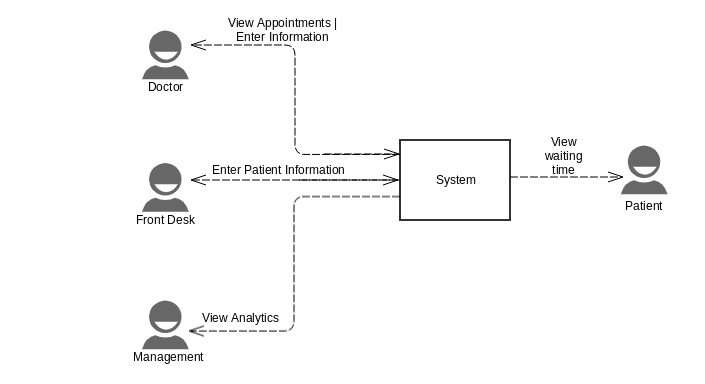
\includegraphics[scale=0.4]{use-case.png}
	\centering
	\caption*{Use case diagram}
\end{figure}

\begin{figure}[h]
	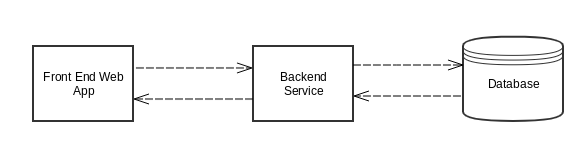
\includegraphics[scale=0.5]{system_architecture.png} 
	\centering
	\caption*{System Architecture}
\end{figure}
\FloatBarrier	


\subsection*{Solution Overview}
The solution is to make a web application that would have features to enlist a patient and assign them to the doctor or department of their choice, record the entry and exit time of a patient into and from the doctors cabin respectively, thereby providing every patient with an waiting time estimated heuristically, which would always be conversative in nature i.e. the estimate would always be less than the actual time to wait, although the discrepancies in the values would be made as minimal as possible. This is done so as to have no effect from the doctors perspective. Ideally the doctor should be oblivious to the use of this technology, and should only have to focus on treating the patients. Thereafter when the waiting time drops below a certain threshold ( say parameter $ \alpha $ ), the patient whose details are captured on the application is sent an immediate ping to report to the counter, wherein if the patient fails to show up after being called within a ( parameter $\beta$ )  few minutes, his/her name on the listing is rescheduled for later. In case, the patient does not arrive despite repeated reschedulings ( parameter $\gamma$ ), their listing for the day is cancelled. Such a system could be in the complete jurisdiction of a receptionist or a staff with a similar posting, but would be available for view to the patients registering. As the application is kept in use for a longer period of time, the heuristics would keep maturing and the estimates would keep getting better, because of the collation of data that continues in the background. There would be an optional feature for the doctor to give an estimate of the amount of time, it would take to look at a patient, based on the history taken. Since there are individual profiles generally stored up on the patient management systems, that information could also provide a graphic to the use case in question, by capturing the patterns with which the patient operates, for eg : whether he/she shows up on time. Generally, hospitals and clinics have a high number of recurring patients thus opening up the opportunity to leverage their \footnote{without stepping on to any private data, focus on recording inocuous information viz. their time of registration, their time of reporting after being pinged to come, and their exact entry and exit times} pattern of behaviour inside the hopsital ergo making the application more robust. As alluded to briefly before, there would be an option of generating a report for the hospital management team, every week or so, to look out for some glaring patterns that debridges their productivity. For example, during festivities factoring in the heavy rush, and deploying more personell to adminster the crowd, or coming to the realization that the waiting time for general physicians is way more than an OPD consult despite there being more traffic at the OPD. Such key insights from the data observed have the potential in assisting the authorities to take better decisions in a bid to achieve the  common goal of improve the quality of service being provided by the hospitals.

\subsection*{Planned Extensions}
A major drawback of the system being proposed is the reliance on a staff at the counter, his/her alertness to collect data. A period of slack off from the staff, wherein no data, or worse false data gets stored has the potential to distort the calculations. Thus it becomes imperative to somehow reduce the dependence on a physical being, and try to automate some of the core processes involved, the first of which pertains to the recording of the exit and entry time. A possible resolution for this, would be control the exit and entry time via a card which is generally provided to a patient whose file is made, after first coming to a hospital or by storing the biometrics of the patient while registering, and having scanners outside of the cabin of the doctor, to record the entry and exit time. Either of the 2 proposed solutions are plausible and the choice of implementation would be dependent on the current system in place. If indeed biometrics are used, then the dependence on a physical being can be completely eradicated. To register, the patient could simply walk up to booths, wherein the application in question would be running, and then on being pinged, they would have to walk up to the booth again, and confirm their presence, thereby preserving the original workflow, but removing the need for an external agent to do the registrations, and replacing it with biometrics to provide the required veritablity. 


\subsection*{Functional Specifications}
\begin{enumerate}
	\item \textbf{Provide an estimate of the waiting time}
	\item \textbf{Option to generate a comprehensive report}
	\item \textbf{Register Patient for Consult}
	\item \textbf{Ping Patient to come to counter}
	\item \textbf{Reschedule for later automatically}
	\item \textbf{Patients view of the data}
\end{enumerate}

\subsection*{Technology Stack}
\begin{enumerate}
	\item \textbf{FrontEnd } : Angular, HTML, CSS, JS
	\item \textbf{Backend} : NodeJS, Express, MongoDB
	\item \textbf{Data Analytics and visualisations} : Python \\
\end{enumerate}
\newpage
\section*{Wireframes}
\begin{figure}[h]

\caption*{Patient's View}
\centering
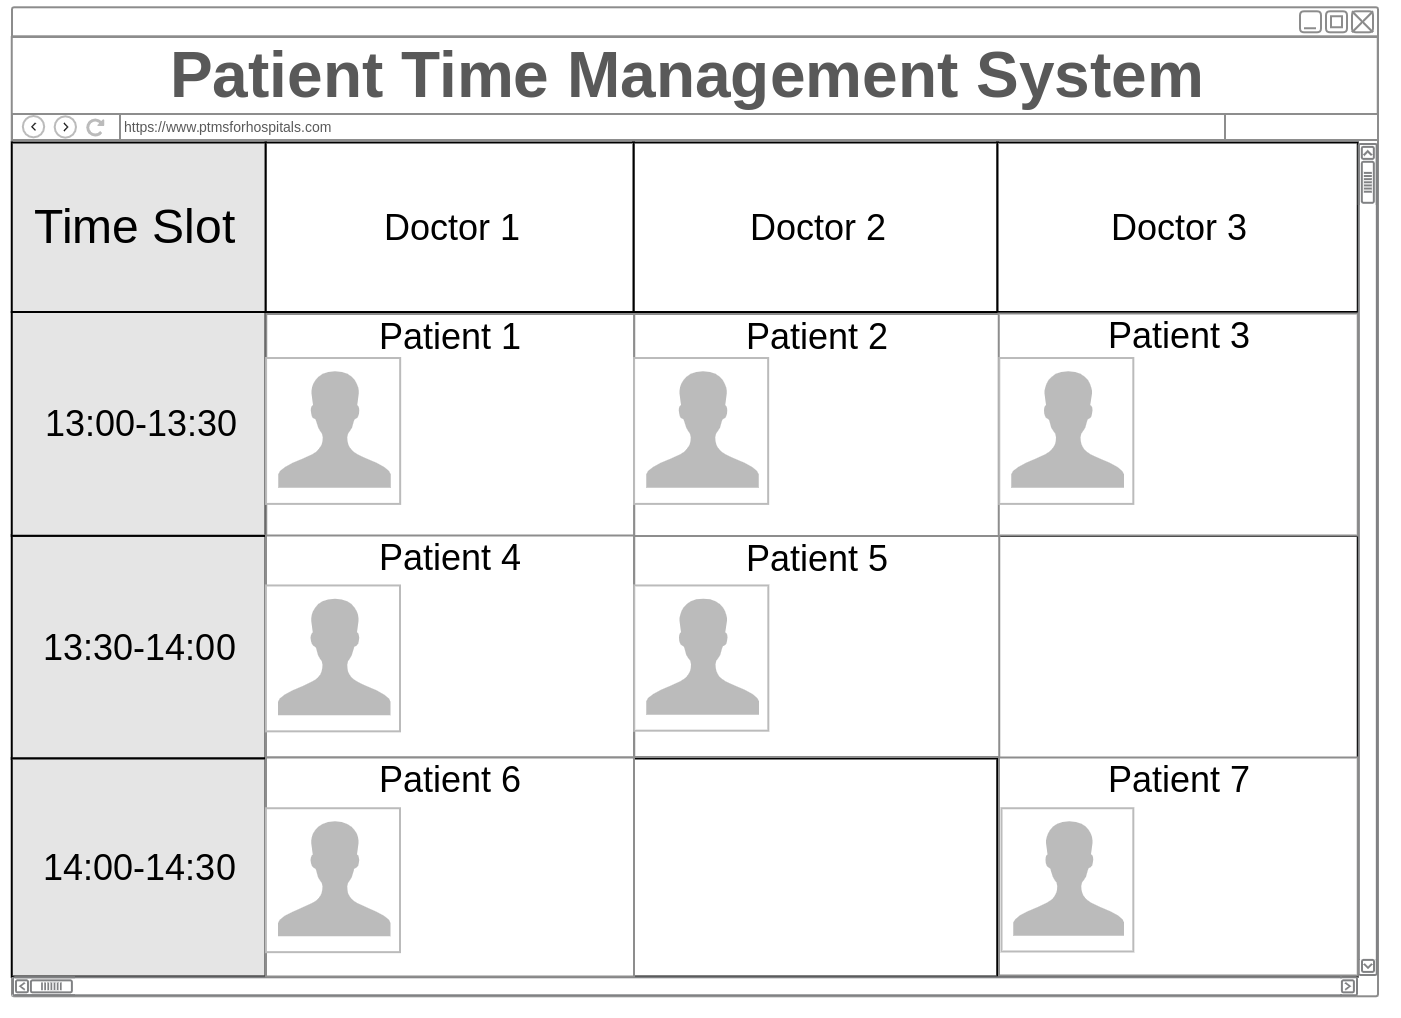
\includegraphics[scale=0.11]{patient.png}
\vspace{3.5mm}
\caption*{Doctor's View}
\centering
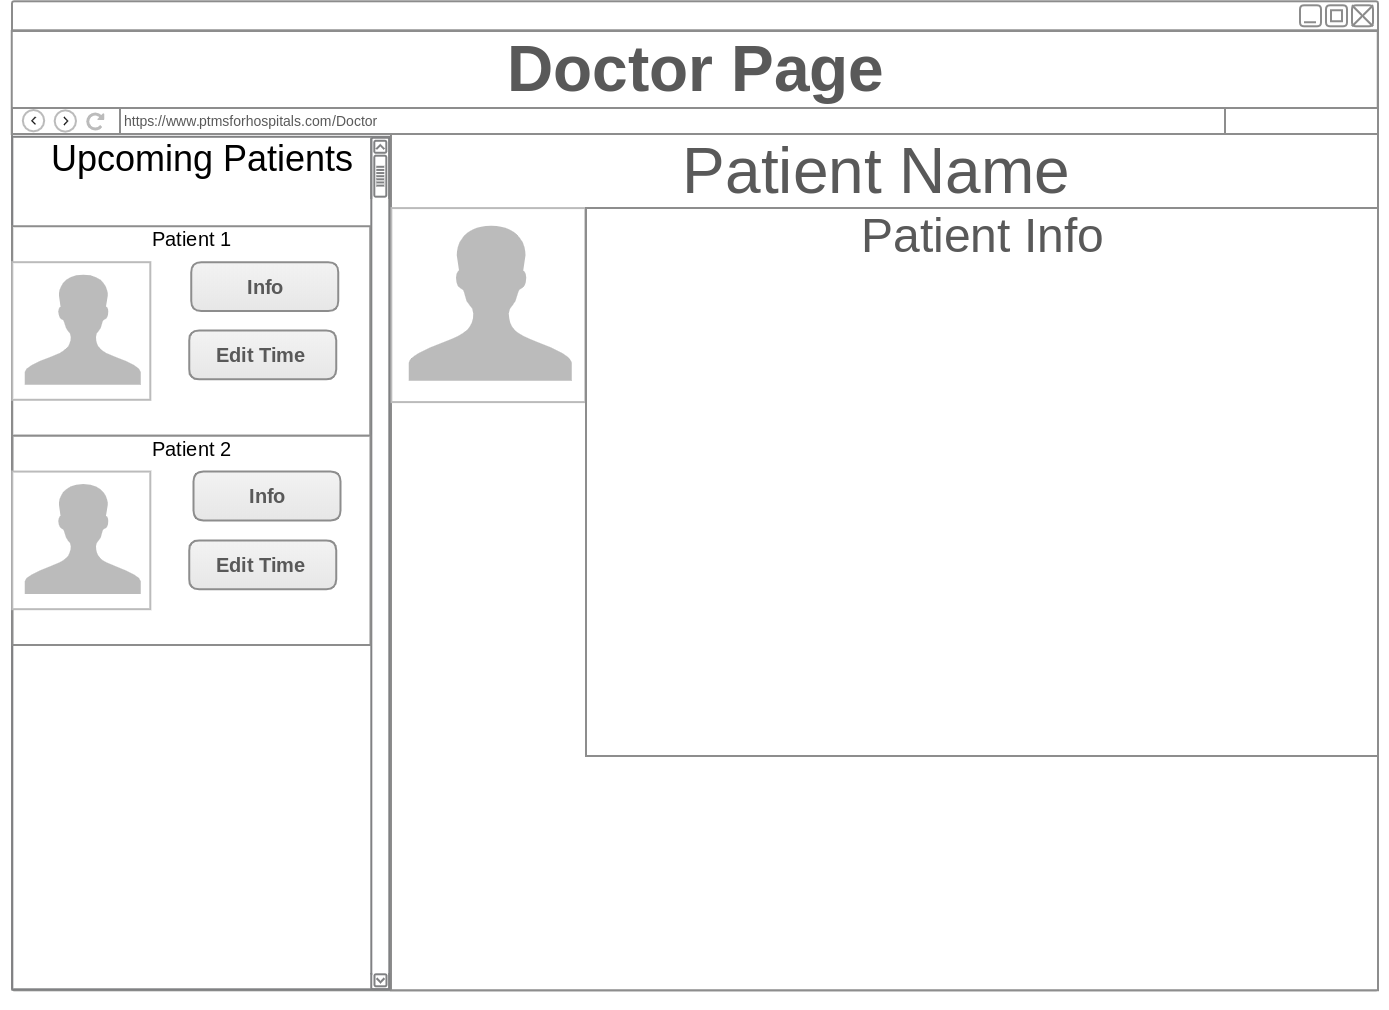
\includegraphics[scale=0.11]{doctor.png}
\vspace{3.5mm}
	\caption*{Reception's View}
	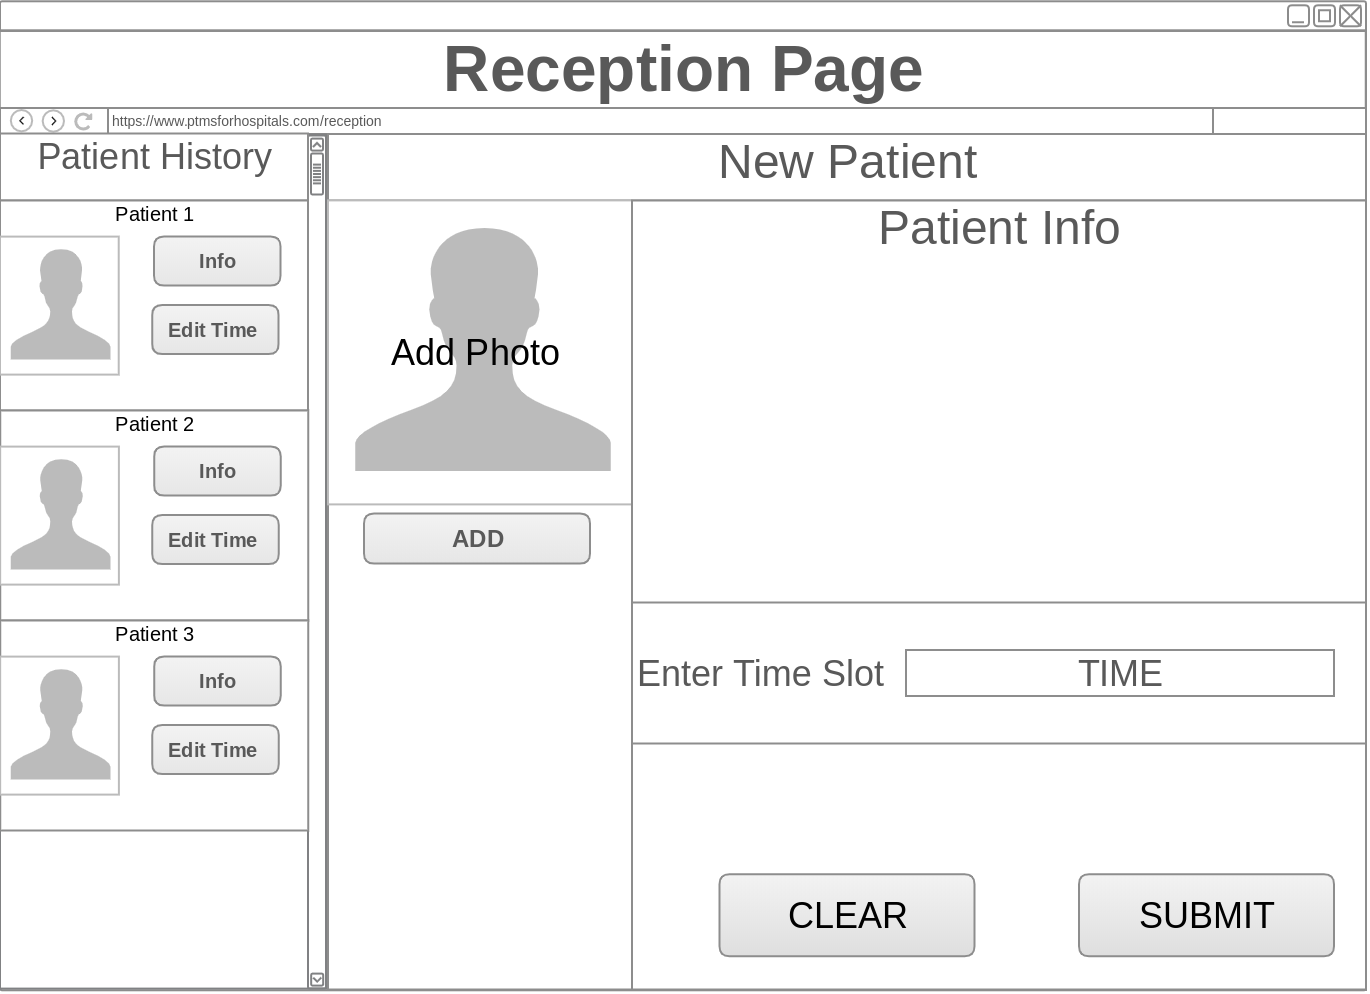
\includegraphics[scale=0.11]{reception.png}
	\centering

\end{figure}

\newpage
\section*{Flow of the Application}

\begin{figure}[h]
	\begin{center}
		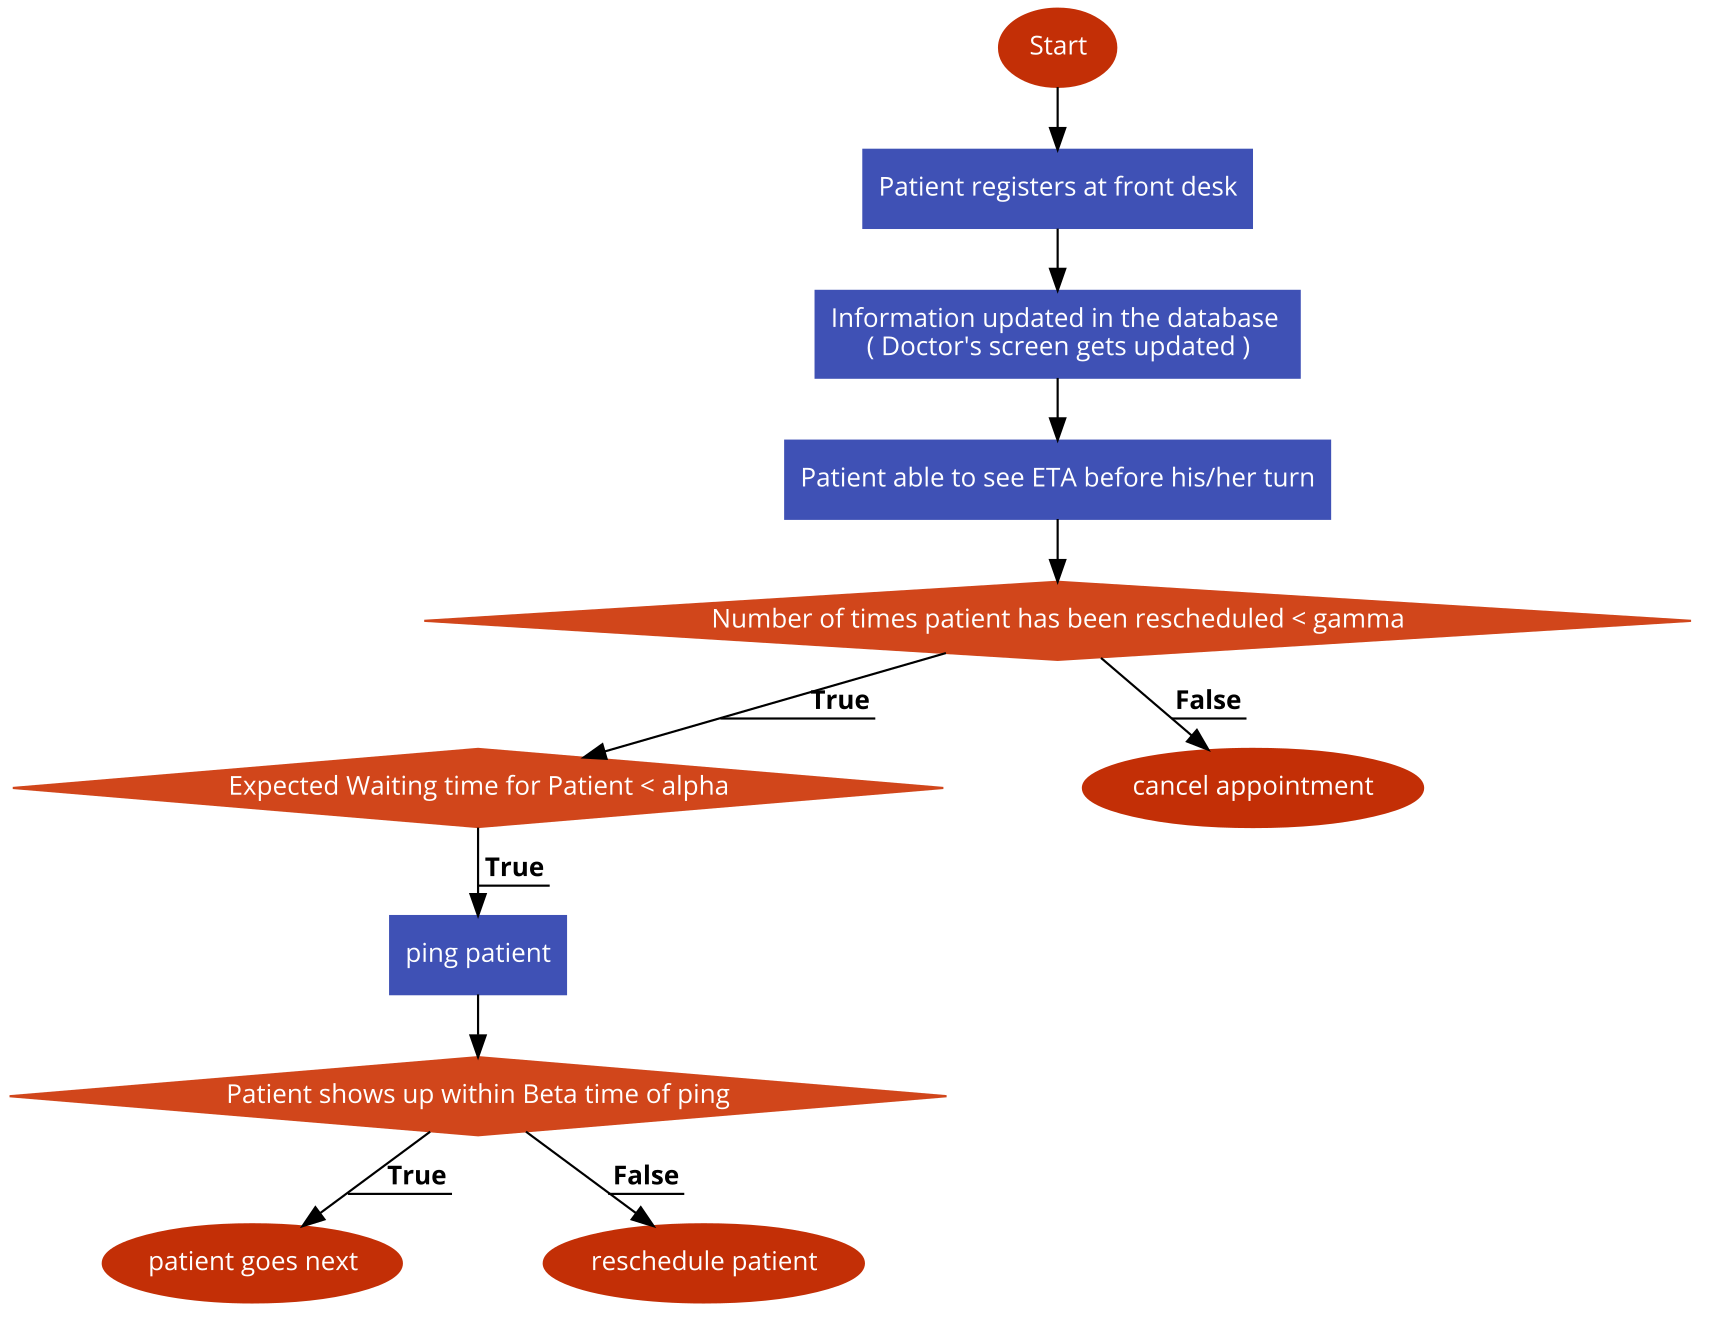
\includegraphics[scale=0.25]{workFlow.png} 
	\end{center}
\end{figure}	

\end{document}


